\begin{exo}
	Dans un pays européen, $12$\% des moutons sont atteints par une maladie.

	Un test de dépistage de cette maladie vient d'être mis sur le marché, mais il n'est pas totalement fiable.

	Une étude a montré que quand le mouton est malade, le test est positif dans 93 \% des cas ; quand le mouton est sain, le test est négatif dans $97$\% des cas.

	On choisit un mouton au hasard et on le soumet au test de dépistage de la maladie.

	On note :
	\begin{itemize}
		\item $M$ l'événement \og{} le mouton est malade \fg{}
		\item $Po$ l'événement \og{} le test est positif \fg{}
	\end{itemize}
	\begin{enumerate}
		\item À l'aide des informations de l'énoncé, donner les valeurs des probabilités suivantes :
		      \[
			      P(M)\ ,\ P_{M}(Po)\ \text{et}\ P_{\overline{M}}(\overline{Po})
		      \]

		\item Compléter l'arbre de probabilité suivant :
	\end{enumerate}
	\begin{center}
		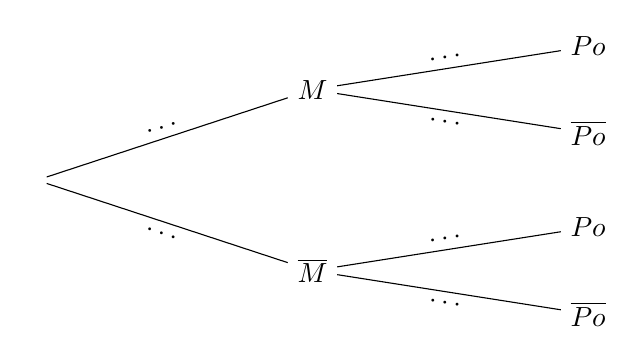
\begin{tikzpicture}[grow=right, sloped, level distance=3.5cm,
				level 1/.style={sibling distance=2.3cm},
				level 2/.style={sibling distance=1.1cm}]

			\node {}
			child {node {$\overline{M}$}
					child {node {$\overline{Po}$} edge from parent node[below] {\dots}}
					child {node {$Po$} edge from parent node[above] {\dots}}
					edge from parent node[below] {\dots}
				}
			child {node {$M$}
					child {node {$\overline{Po}$} edge from parent node[below] {\dots}}
					child {node {$Po$} edge from parent node[above] {\dots}}
					edge from parent node[above] {\dots}
				};

		\end{tikzpicture}
	\end{center}

	\begin{enumerate}[resume]
		\item Calculer $P\pa{M\cap Po}$ et interpréter le résultat dans le cadre de l'exercice.
		\item Calculer la probabilité que le mouton soit sain et que son test soit négatif.
	\end{enumerate}
\end{exo}
